% \chapter{Path tracking}
	\section{Path tracking, Modeling exercise}
		%
		Automated vehicles must follow paths that the vehicles' own decision-making layers generate to enable the vehicle to stay in its lane, change lanes, cross intersections, avoid collisions, etc. 
		Some path-tracking methods found in the literature tackle the challenge by exploiting a kinematic model of the vehicle that describes the vehicle's position w.r.t.\ to the path that is to be tracked.

		Consider a reference path defined by a function %
		$\pi : \mathbb{R}\to\mathbb{R}^3$, %
		that, given a distance %
		$s_\pi\in\mathbb{R}$ %
		along the path, outputs a tuple %
		$(x_\pi(s_\pi), y_\pi(s_\pi), \theta_\pi(s_\pi))$ %
		representing the x-y position %
		$(x_\pi(s_\pi), y_\pi(s_\pi))$, %
		and orientation %
		$\theta_\pi(s_\pi)$ %
		at %
		$s_\pi$. %
		Then, given a point %
		$P_r\in\mathbb{R}^2$ %
		positioned in the middle of the vehicle's rear bumper, and the point %
		$P_{r,\pi}\in\mathbb{R}^2$ %
		corresponding to the projection of %
		$P_r$ %
		in the path %
		$\pi$, %
		the position of a vehicle could be described by:
		\begin{itemize}
			\item the distance %
			$\pathCoor\in\mathbb{R}$ %
			along the path corresponding to the vehicle's projections, 
			\item the so-called \emph{lateral error} %
			$d\in\mathbb{R}$, %
			defined as %
			$d = ||P_r - P_{r,\pi}||$, %
			showing the distance to the path, and
			\item the so-called \emph{heading error} %
			$\theta_e \in \mathbb{R}$, %
			defined as %
			$\theta_e = (\theta - \theta_\pi)$, %
			showing the difference between the vehicle's yaw angle $\theta$ and the path's orientation %
			$\theta_\pi$ at $P_{r,\pi}$. 
 		\end{itemize}
 		The coordinates listed above are illustrated in Fig.\ \ref{fig:system}.

		\begin{figure}[!h]
			\centering
			\resizebox{ 300 px }{!}{
				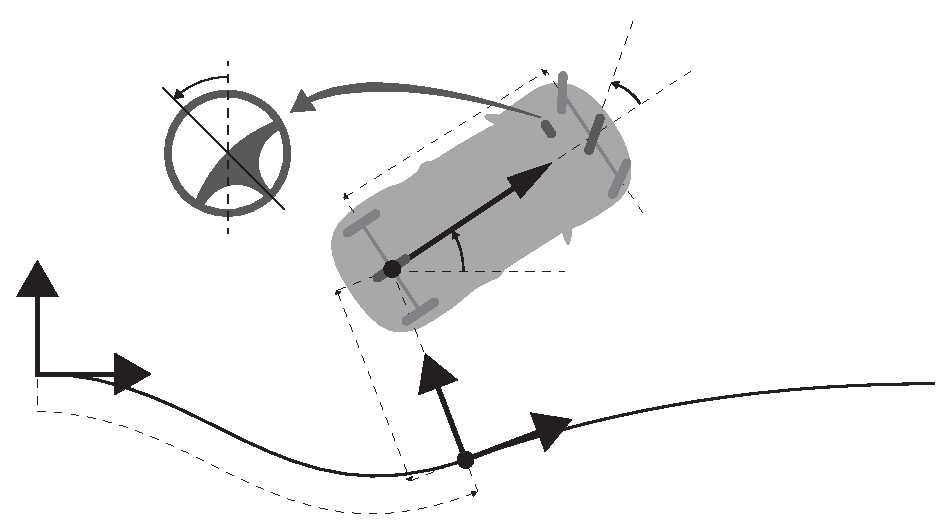
\includegraphics[width = 250px]{./_imags/system}
				\put(-187,0){$\pathCoor$}
				\put(-163,30){$\distToPath$}
				% \put(-55,110){$\yawErr$}
				\put(-85,120){$\frac{\steering}{16}$}
				\put(-205,121){$\steering$}
				\put(-127,70){$\yaw$}
				\put(-162,68){$P_r$}
				\put(-132,85){$\speed$}
				\put(-142,105){$\carLength$}
				\put(-128,05){$P_{r,\pi}$}
				\put(-28,38){$\pi$}
			}
			\caption{Coordinate system.}
			\label{fig:system}
		\end{figure}	
		%
		
		Representing by %
		$\phi\in\mathbb{R}$ %
		the position of the steering wheel (measured in radians), and assuming our control inputs to be the longitudinal speed reference %
		$v_{ref}\in\mathbb{R}^+$ %
		and the steering wheel's position reference %
		$\phi_{ref}\in[-4\pi, 4\pi]$, %
		the vehicle's model can be formulated as follows:
		\begin{subequations}
		\begin{align}	
			\dpathCoor 	& = \frac{\speed\cos(\yawErr)}{1-\distToPath\curvature} 
			\label{eq:non_linear_model_1}\\
			\ddistToPath& = \speed\sin(\yawErr) 
			\label{eq:non_linear_model_2}\\
			\dyawErr    & = \frac{\speed}{\carLength}\tan(\steering/16 ) - \curvature\dpathCoor 
			\label{eq:non_linear_model_3}\\
			\dspeed & = \accDyn(\speed_{ref}-\speed) 
			\label{eq:non_linear_model_4}\\
			\dsteering & = \steerDyn(\steering_{ref}-\steering) 
			\label{eq:non_linear_model_5}
		\end{align}
		\end{subequations}
		where %
		$\curvature$ %
		denotes the curvature of the path at %
		$\pathCoor$, %
		and %
		$\accDyn$ %
		and %
		$\steerDyn$ %
		represent the dynamic with which the speed and steering wheel references are followed.
		For the sake of further simplicity, from now on we will assume that the path has a constant curvature, i.e.\ %
		$\curvature = \kappa$. 
		\par
		%
		The states and control inputs of our system are
		\begin{align}
			\mathbf{\state} & = 
				\left[ \stat{1},\stat{2},\stat{3},\stat{4},\stat{5}\right] = %
				\left[\pathCoor, \distToPath, \yawErr, \speed, \steering\right] \label{eq:stateVector}, \\ 
			\mathbf{\control} & = 
				\left[ \con{1},\con{2} \right] = %
				\left[ \speed_{ref}, \steering_{ref} \right].
		\end{align}
		% which allows us writing the model in the form $ \mathbf{\dot{\state}} = f(\mathbf{\state},\mathbf{\control}) $ as
		% \begin{align}
		% 	%
		% 	%\dstat{1} 	& = \stat{7}\cos(\stat{3})\\
		% 	%\dstat{2} 	& = \stat{7}\sin(\stat{3})\\
		% 	%\dstat{3} 	& = \frac{\stat{7}}{L}\tan{\stat{8}}\\
		% 	%
		% 	\dstat{1} 	& = \frac{\stat{4}\cos(\stat{3})}{1-\stat{2}\curv} \label{eq:ss1}\\
		% 	\dstat{2}   & = \stat{4}\sin(\stat{3}) \label{eq:ss2}\\
		% 	\dstat{3}   & = \frac{\stat{4}}{\carLength}\tan(\stat{5}) - \frac{\curv\stat{4}\cos(\stat{3})}{1-\stat{2}\curv} \label{eq:ss3}\\
		% 	% \dstat{4}   & = \accDyn(\con{1}-\stat{4})\label{eq:ss4}\\
		% 	% \dstat{5}   & = \steerDyn(\con{2}-\stat{5}) \label{eq:ss5}
		% 	\dstat{4}   & = u_1\label{eq:ss4}\\
		% 	\dstat{5}   & = u_2 \label{eq:ss5}		
		% \end{align}
		% %
		% which is the system's continuous non-linear model we will use to design and implement the studied control and observation techniques. 
			
		Moreover, unless stated otherwise, we will consider the output of the system to be 
		\begin{align}
			\mathbf{y} = \mathbf{x}.
		\end{align}

		Answer the following questions:
		\begin{itemize}
			\item Rewrite the non-linear model in the standard form $\mathbf{\dot{\state}} = f(\mathbf{\state},\mathbf{\control})$.
			\item Given the chosen state space, why it wouldn't be appropriate linearizing the system around a nominal \emph{point}.
			\item Calculate the \emph{nominal trajectory} representing the constant-speed perfect tracking situation (that is, a situation where the vehicle drives perfectly on the path and at a constant speed %
			$v_{ref}$) for a path of constant curvature $\curv_{ref}$. 
			\item Linearize the system around such a nominal trajectory.
			\item Discretize the system using Euler approximation. 
		\end{itemize}

% \newpage
% 	\section{Solution}
% 		\subsection{Non linear model}
% 			Let's begin rewriting the non linear model in standard form. 
% 			\begin{align}
% 				\dstat{1} & = f_1(\mathbf{x}, \mathbf{u}) =
% 					\frac{\stat{4}\cos(\stat{3})}{1-\stat{2}\curv_{ref}} \label{nl:01}\\
% 				\dstat{2} & = f_2(\mathbf{x}, \mathbf{u}) =
% 					\stat{4}\sin(\stat{3})\label{nl:02}\\
% 				\dstat{3} & = f_3(\mathbf{x}, \mathbf{u}) =
% 					\frac{\stat{4}}{\carLength}\tan(\stat{5}/16) - \frac{\curv_{ref}\stat{4}\cos(\stat{3})}{1-\stat{2}\curv_{ref}}\label{nl:03}\\
% 				\dstat{4} & = f_4(\mathbf{x}, \mathbf{u}) =
% 					\sigma_v (u_1 -  x_4) \label{nl:04}\\
% 				\dstat{5} & = f_5(\mathbf{x}, \mathbf{u}) =
% 					\sigma_\phi(u_2 - x_5) \label{nl:05}
% 			\end{align}
% 		\subsection{Why not working point?}
% 			Typically, the working point is calculated by doing %
% 			$\dot{\mathbf{x}} = 0$. %
% 			However, as $\state_1$ represents the location of the projection of the vehicle's position in the path, making %
% 			$\dot{\state}_1=0$ %
% 			would describe a situation where $\state_1$ is fixed, thus where the vehicle does not move forward. 

% 			Then, as in the nominal situation $\state_1$ must evolve over time, the system must be linearized around a nominal \emph{trajectory} and not a nominal \emph{point}.

% 		\subsection{Nominal trajectory}
% 			To linearize the system, we first need to define the nominal trajectory $\overline{\mathbf{x}}(t)$. 
% 			As the path tracking is said to be perfect and at constant speed, we know that
% 			\begin{align}
% 				\dot{\bx}_1(t) &= v_{ref}, &
% 				\dot{\bx}_2(t) &= 0, & 
% 				\dot{\bx}_3(t) &= 0, & 
% 				\dot{\bx}_4(t) &= 0, & 
% 				\dot{\bx}_5(t) &= 0.
% 			\end{align}
% 			The nominal trajectory then results from solving the system of equations $
% 			\dot{\overline{\mathbf{x}}} = f(\overline{\mathbf{x}}, \overline{\mathbf{u}})$.
% 			Specifically
% 			\begin{align}
% 				v_{ref} & = \frac{\bx_{4}\cos(\bx_{3})}{1-\bx_{2}\curv_{ref}}\label{lm:01}\\
% 				0 & = \bx_{4}\sin(\bx_{3})\\
% 				0 & = \frac{\bx_{4}}{\carLength}\tan(\bx_{5}/16) - 
% 					\frac{\curv_{ref}\bx_{4}\cos(\bx_{3})}{1-\bx_{2}\curv_{ref}}\label{lm:03}\\
% 				\overline{x}_4 & = \overline{u}_1\\
% 				\overline{x}_5 & = \overline{u}_2.
% 			\end{align}
% 			On the one hand, we note that $\bx_1$ does not appear on the set of equations above. 
% 			However, as its derivative must be $v_{ref}$ we can obtain its value
% 			\begin{align}
% 				\bx_1(t) & = v_{ref} t + x_1(t_0).
% 			\end{align}
% 			Then, as we stated the nominal trajectory must be perfect, both the lateral and the heading deviation must be zero in the nominal state, i.e.\ $\bx_2(t) = 0$ and $\bx_3(t) = 0$.
% 			From Eq.\ \ref{lm:01}, we obtain $\bx_4(t) = v_{ref}$.
% 			From Eq.\ \ref{lm:03} we have that
% 			\begin{align}
% 				0 & = \frac{v_{ref}}{\carLength}\tan(\bx_{5}) - 
% 					\curv_{ref} v_{ref},
% 			\end{align}
% 			thus, 
% 			\begin{align}
% 				\bx_{5} = 16\arctan(\carLength\curv_{ref}).
% 			\end{align}
% 			Then, the nominal trajectory is
% 			\begin{align}
% 				\overline{\mathbf{x}}(t) & = [
% 					v_{ref} t + x_1(t_0),\quad 
% 					0,\quad
% 					0,\quad
% 					v_{ref},\quad
% 					16\arctan(\carLength\curv_{ref})]\\
% 				\overline{\mathbf{u}}(t) & = [
% 					v_{ref}, \quad 16\arctan(\carLength\curv_{ref})]
% 			\end{align}

% 		\subsection{Linearization}	
% 			To linearize the system we need to calculate the terms of the Taylor series expansion of the non linear equations of our model. 
% 			For Eq.\ \ref{nl:01} we have
% 			\begin{align}
% 				\frac{\partial f_1}{\partial x_1}(\overline{\mathbf{x}}, \overline{\mathbf{u}}) & 
% 					= 0, &
% 				\frac{\partial f_1}{\partial x_2}(\overline{\mathbf{x}}, \overline{\mathbf{u}}) & 
% 					= \frac{\bx_4 \cos(\bx_3)\curv_{ref}}{ (1-\bx_2 \curv_{ref})^2 }, &
% 				\frac{\partial f_1}{\partial x_3}(\overline{\mathbf{x}}, \overline{\mathbf{u}}) & 
% 					= -\frac{\bx_4 \sin(\bx_3)}{1-\bx_2\curv_{ref}}, \\
% 				\frac{\partial f_1}{\partial x_4}(\overline{\mathbf{x}}, \overline{\mathbf{u}}) & 
% 					= \frac{\cos(\bx_3)}{1-\bx_2\curv_{ref}}, &
% 				\frac{\partial f_1}{\partial x_5}(\overline{\mathbf{x}}, \overline{\mathbf{u}}) & 
% 					= 0, &
% 				\frac{\partial f_1}{\partial u_1}(\overline{\mathbf{x}}, \overline{\mathbf{u}}) & 
% 					= 0,\\
% 				\frac{\partial f_1}{\partial u_2}(\overline{\mathbf{x}}, \overline{\mathbf{u}}) & 
% 					= 0. & & & & 
% 			\end{align}
% 			For Eq.\ \ref{nl:02} we have
% 			\begin{align}
% 				\frac{\partial f_2}{\partial x_1}(\overline{\mathbf{x}}, \overline{\mathbf{u}}) & 
% 					= 0, &
% 				\frac{\partial f_2}{\partial x_2}(\overline{\mathbf{x}}, \overline{\mathbf{u}}) & 
% 					= 0, &
% 				\frac{\partial f_2}{\partial x_3}(\overline{\mathbf{x}}, \overline{\mathbf{u}}) & 
% 					= \bx_4\cos(\bx_3), &
% 				\frac{\partial f_2}{\partial x_4}(\overline{\mathbf{x}}, \overline{\mathbf{u}}) & 
% 					= \sin(\bx_3),\\
% 				\frac{\partial f_2}{\partial x_5}(\overline{\mathbf{x}}, \overline{\mathbf{u}}) & 
% 					= 0, &
% 				\frac{\partial f_2}{\partial u_1}(\overline{\mathbf{x}}, \overline{\mathbf{u}}) & 
% 					= 0, &
% 				\frac{\partial f_2}{\partial u_2}(\overline{\mathbf{x}}, \overline{\mathbf{u}}) & 
% 					= 0. & & 
% 			\end{align}
% 			For Eq.\ \ref{nl:03} we have
% 			\begin{align}
% 				\frac{\partial f_3}{\partial x_1}(\overline{\mathbf{x}}, \overline{\mathbf{u}}) & 
% 					= 0, &
% 				\frac{\partial f_3}{\partial x_2}(\overline{\mathbf{x}}, \overline{\mathbf{u}}) & 
% 					= -\frac{\curv_{ref}\bx_4\cos(\bx_3)\curv_{ref}}{(1-x_2\curv_{ref})^2}, \\
% 				\frac{\partial f_3}{\partial x_3}(\overline{\mathbf{x}}, \overline{\mathbf{u}}) & 
% 					= \frac{\curv \bx_4 \sin(\bx_3)}{1-\bx_2\curv_{ref}}, & 
% 				\frac{\partial f_3}{\partial x_4}(\overline{\mathbf{x}}, \overline{\mathbf{u}}) & 
% 					= \frac{\tan(x_5/16)}{L} - \frac{\curv \cos(\bx_3)}{1 - \bx_2 \curv_{ref}}, \\
% 				\frac{\partial f_3}{\partial x_5}(\overline{\mathbf{x}}, \overline{\mathbf{u}}) & 
% 					= \frac{x_4}{16L\cos(x_5/16)^2}, &
% 				\frac{\partial f_3}{\partial u_1}(\overline{\mathbf{x}}, \overline{\mathbf{u}}) & 
% 					= 0,\\
% 				\frac{\partial f_3}{\partial u_2}(\overline{\mathbf{x}}, \overline{\mathbf{u}}) & 
% 					= 0. & & 
% 			\end{align}
% 			For Eq.\ \ref{nl:04} we have
% 			\begin{align}
% 				\frac{\partial f_4}{\partial x_1}(\overline{\mathbf{x}}, \overline{\mathbf{u}}) & 
% 					= 0, &
% 				\frac{\partial f_4}{\partial x_2}(\overline{\mathbf{x}}, \overline{\mathbf{u}}) & 
% 					= 0, &
% 				\frac{\partial f_4}{\partial x_3}(\overline{\mathbf{x}}, \overline{\mathbf{u}}) & 
% 					= 0, & 
% 				\frac{\partial f_4}{\partial x_4}(\overline{\mathbf{x}}, \overline{\mathbf{u}}) & 
% 					= -\sigma_v,\\
% 				\frac{\partial f_4}{\partial x_5}(\overline{\mathbf{x}}, \overline{\mathbf{u}}) & 
% 					= 0, &
% 				\frac{\partial f_4}{\partial u_1}(\overline{\mathbf{x}}, \overline{\mathbf{u}}) & 
% 					= \sigma_v, &
% 				\frac{\partial f_4}{\partial u_2}(\overline{\mathbf{x}}, \overline{\mathbf{u}}) & 
% 					= 0. & &
% 			\end{align}
% 			For Eq.\ \ref{nl:05} we have
% 			\begin{align}
% 				\frac{\partial f_5}{\partial x_1}(\overline{\mathbf{x}}, \overline{\mathbf{u}}) & 
% 					= 0, &
% 				\frac{\partial f_5}{\partial x_2}(\overline{\mathbf{x}}, \overline{\mathbf{u}}) & 
% 					= 0, &
% 				\frac{\partial f_5}{\partial x_3}(\overline{\mathbf{x}}, \overline{\mathbf{u}}) & 
% 					= 0, &
% 				\frac{\partial f_5}{\partial x_4}(\overline{\mathbf{x}}, \overline{\mathbf{u}}) & 
% 					= 0,\\
% 				\frac{\partial f_5}{\partial x_5}(\overline{\mathbf{x}}, \overline{\mathbf{u}}) & 
% 					= -\sigma_\phi, &
% 				\frac{\partial f_5}{\partial u_1}(\overline{\mathbf{x}}, \overline{\mathbf{u}}) & 
% 					= 0, &
% 				\frac{\partial f_5}{\partial u_2}(\overline{\mathbf{x}}, \overline{\mathbf{u}}) & 
% 					= \sigma_\phi. & &
% 			\end{align}

% 			Then the Jacobian matrix will be 
% 			\begin{align}
% 				A & = \left(
% 				\begin{array}{ccccc}
% 					0 & 
% 					\frac{\bx_4 \cos(\bx_3)\curv_{ref}}{ (1-\bx_2 \curv_{ref})^2 } & 
% 					-\frac{\bx_4 \sin(\bx_3)}{1-\bx_2\curv_{ref}} & 
% 					\frac{\cos(\bx_3)}{1-\bx_2\curv_{ref}} & 
% 					0 \\
% 					%
% 					0 &
% 					0 &
% 					\bx_4\cos(\bx_3) &
% 					\sin(\bx_3) &
% 					0 \\ 
% 					%
% 					0 &
% 					-\frac{\curv_{ref}\bx_4\cos(\bx_3)\curv_{ref}}{(1-x_2\curv_{ref})^2} &
% 					\frac{\curv \bx_4 \sin(\bx_3)}{1-\bx_2\curv_{ref}} &
% 					\frac{\tan(x_5/16)}{L} - \frac{\curv \cos(\bx_3)}{1 - \bx_2 \curv_{ref}} &
% 					\frac{x_4}{16L\cos(x_5/16)^2} \\
% 					%
% 					0 &
% 					0 &
% 					0 &
% 					-\sigma_v &
% 					0 \\
% 					%
% 					0 &
% 					0 &
% 					0 &
% 					0 &
% 					-\sigma_\phi 
% 				\end{array}
% 				\right) = \\
%  				& = \left(
% 				\begin{array}{ccccc}
% 					0 & 
% 					v_{ref}\curv_{ref} & 
% 					0 & 
% 					1 & 
% 					0 \\
% 					%
% 					0 &
% 					0 &
% 					v_{ref} &
% 					0 &
% 					0 \\ 
% 					%
% 					0 &
% 					-\curv_{ref}^2v_{ref} &
% 					0 &
% 					0 &
% 					\frac{v_{ref}}{16L\cos(\arctan(\carLength\curv_{ref}))^2} \\
% 					%
% 					0 &
% 					0 &
% 					0 &
% 					-\sigma_v&
% 					0 \\
% 					%
% 					0 &
% 					0 &
% 					0 &
% 					0 &
% 					-\sigma_\phi
% 				\end{array}
% 				\right) = \\
%  				& = \left(
% 				\begin{array}{ccccc}
% 					0 & 
% 					v_{ref}\curv_{ref} & 
% 					0 & 
% 					1 & 
% 					0 \\
% 					%
% 					0 &
% 					0 &
% 					v_{ref} &
% 					0 &
% 					0 \\ 
% 					%
% 					0 &
% 					-\curv_{ref}^2v_{ref} &
% 					0 &
% 					0 &
% 					\frac
% 					{v_{ref} + v_{ref}\carLength^2\curv_{ref}^2}
% 					{16L}\\
% 					%
% 					0 &
% 					0 &
% 					0 &
% 					-\sigma_v &
% 					0 \\
% 					%
% 					0 &
% 					0 &
% 					0 &
% 					0 &
% 					-\sigma_\phi
% 				\end{array}
% 				\right).
% 			\end{align}
% 			Furthermore
% 			\begin{align}
% 				b = \left(
% 				\begin{array}{cc}
% 					0 & 0 \\
% 					0 & 0 \\
% 					0 & 0 \\
% 					\sigma_v & 0 \\
% 					0 & \sigma_\phi
% 				\end{array}
% 				\right)
% 			\end{align}.
% 			Finally
% 			\begin{align}
% 				c = \left(
% 				\begin{array}{ccccc}
% 					1 & 0 & 0 & 0 & 0 \\
% 					0 & 1 & 0 & 0 & 0 \\
% 					0 & 0 & 1 & 0 & 0 \\
% 					0 & 0 & 0 & 1 & 0 \\
% 					0 & 0 & 0 & 0 & 1
% 				\end{array}
% 				\right)
% 			\end{align}
% 		\subsection{Euler discretization}
% 			The Euler approximation consists of approximating the states derivative by 
% 			\begin{align}
% 				\dot{x} = \frac{x(k+1)-x(k)}{h}.
% 			\end{align}
% 			Then, from the standard form 
% 			\begin{align}
% 				\dot{\mathbf{x}} & = A \mathbf{x} + B \mathbf{u}\\
% 				\mathbf{y} & = C \mathbf{x} + D \mathbf{u}
% 			\end{align}
% 			we would have
% 			\begin{align}
% 				\frac{\mathbf{x}(k+1)-\mathbf{x}(k)}{h} & = A \mathbf{x}(k) + B \mathbf{u}(k)\\
% 				\mathbf{x}(k+1)-\mathbf{x}(k) & = hA \mathbf{x}(k) + hB \mathbf{u}(k)\\
% 				\mathbf{x}(k+1) & = \mathbf{I}\mathbf{x}(k) + hA \mathbf{x}(k) + hB \mathbf{u}(k)\\
% 				\mathbf{x}(k+1) & = (\mathbf{I} + hA)\mathbf{x}(k) + hB \mathbf{u}(k)\\
% 			\end{align}


%             % A(1,2) = vr*k;
%             % A(1,4) = 1;
%             % A(2,3) = vr;
%             % A(3,2) = -vr*k^2;
%             % A(3,5) = vr*(1+k^2*L^2)/L;
%             % A(4,4) = -parameters(3);
%             % A(5,5) = -parameters(4);			
% \newpage
